\chapter{绪论}
%\section{安装\LaTeX{} }
%\subsection{Mac OS X}
%\begin{figure}[htbp]
%\centering\includegraphics[width=5cm,height=1.32cm]{figures/Logo_2.pdf}
%\caption[示意图]{用LaTeX画图}
%\end{figure}

\section{研究背景与意义}
随着移动互联网的快速发展,人们可以随时随地通过智能设备上的应用创建和分享各种不同模态的多媒体数据,如文本、图像、视频等。其中视频
数据具有更丰富的信息,受到了更多用户的青睐,据《第44次中国互联网络发展状况统计报告》~\footnote{\url{http://www.cac.gov.cn/2019-08/30/c\_1124938750.htm}}显示,截至2019年6月,我国的网络视频用户规模
达7.59亿,占网民整体的88.8\%,其中短视频用户规模为6.48亿,占网民整体的75.8\%。各种短视频的智能设备应用也是呈井喷式的发展,如抖音、
快手等应用,用户可以通过这些应用创建和分享一分钟以内的短视频,据《2019年抖音数据报告》~\footnote{\url{https://weibo.com/ttarticle/p/show?id=2309404457716281114897}}显示,截至2020年1月5日,抖音日活跃用户数已经超过4亿,而根据快手发布的《2019快手内容报告》~\footnote{\url{http://www.chinanews.com/business/2020/02-22/9100846.shtml}}
显示,2019年有2.5亿用户通过快手平台发布作品,平台内有近200亿条的海量视频数据。在如此庞大的并且还在快速增长的视频数据里,
如何高效和精确地检索出用户需要或者感兴趣的视频是一个具有很大挑战并且具有应用价值的问题,是多媒体检索领域内的热点问题~\cite{hong2017,geetha2008a,hu2011a,peng2018an}。

即席视频检索检索(Ad-hoc Video Search, AVS)是指用户根据自己的需求以句子的形式来查询未经标注的视频,例如“一个有胡子的男人对着麦克风讲话或唱歌”~\cite{awad2016trecvid}。这和经典的基于内容的视频检索~\cite{yu2015content}不同,基于内容的视频检索是以一个图像或者视频片段
作为查询,从候选的视频数据中检索出与该查询内容相同或者相似的视频。这种视频检索方式在实际应用中有很大的局限性,因为用户通常不具有
能够表达其查询需求的图片或者视频,而以句子的形式表达用户需求则是一种更加直接方便的方式,例如用户希望检索出“一个男人在唱歌”这样场景的视频,而其并没有这样的样例视频,则其不能通过这种基于视频内容的视频检索技术进行检索,因此用户会更加倾向于使用句子的形式作为查询来检索想要的视频。即席视频检索也不同于长期研究的基于概念的视频检索技术~\cite{snoekcees2009concept},这种检索技术的和核心是从视频中
检测出某些特定的概念,例如视频中出现的人或者物体,然后对查询句子提取关键词,利用查询关键词与检测出的概念进行匹配,这种检索技术需要
先定义一个概念集,然后检测视频中出现的概念,因此检索效果受限于概念的选择并且这种技术对查询句子的语义也没有进行建模分析。而本文研究
的即席视频检索是解决用户以一种模态的多媒体对象(文本)作为查询输入,检索出与查询语义上相同或相近的另一种模态的多媒体对象(视频),
这本质是也是一直被广泛关注的跨模态检索技术~\cite{rasiwasia2010a,feng2014cross,pereira2014on,suris2018cross,mithun2018learning}。
即席视频检索的核心是计算查询文本与候选视频在语义上的相关度,然后根据该相关度对候选视频进行排序,从而从候选视频中选出用户期望的视频,图~\ref{fig:fig_1}展示了即席视频检索的大致流程。由于查询文本与视频是两种不同的模态,它们在底层表示上是异构的,即文本是由一序列的单词排列组成,而视频是由一序列图像组成并且伴随着音频,这也通常被称为“异构鸿沟”,因此这两种数据是不能直接进行比较或者计算相关度的。这两种
媒体数据的异构性和不可比性,使得即席视频检索是一个非常具有挑战性的研究任务。得益于美国国家标准与技术研究院(National Institute of Standards and Technology, NIST)举行的视频检索国际权威评测TRECVID AVS,提供的大量的测试数据集合、统一的评价标准,吸引了来自包括卡内基梅隆大学、弗吉尼亚大学、香港中文大学、早稻田大学等全球各地的优秀学者参与评测,推动了即席视频检索技术的发展~\cite{awad2016trecvid,awad2017trecvid,awad2018trecvid,awad2019trecvid}。如表格\ref{tab:method-diffs}所示,最近四年的研究方法都是基于公共空间学习的方法,这种方法为文本和视频学习一个公共空间,并将这两种模态的数据投影到公共空间进行表示,使得这两种数据的相关度可以在这个公共空间通过直接计算距离进行衡量,
这种方法有三个关键的模块,即文本表示、视频表示和公共空间,这三个模块的好坏与检索算法的效果有直接的关系,本文将关注对文本表示和公共空间这两个模块的改进,而视频表示则采用简单但有效的通过预训练的卷积神经网络(ResNeXt-101, ResNet-152)提取的视觉特征~\cite{li2018renmin,li2019renmin}。

\begin{figure*}[tbh!]
    \centering
    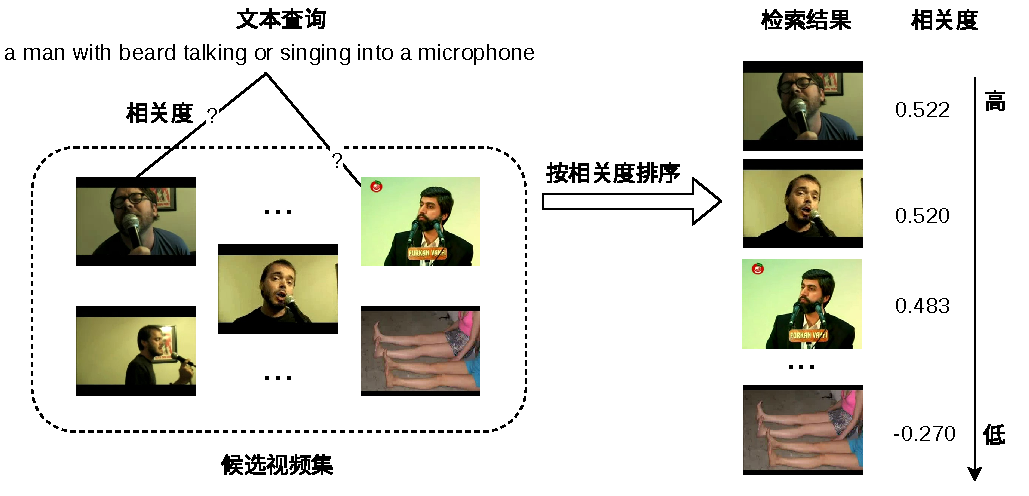
\includegraphics[width=\linewidth]{figures/1}
    \caption[即席视频检索流程]{\textbf{即席视频检索流程。即席视频检索技术首先计算查询与候选视频的相关度,然后根据相关度对候选视频进行排序,从而得到最终的视频检索结果。本文使用余弦相似度来度量查询与候选视频的相关度,范围从-1到1,余弦相似度越大,则表明查询与候选视频的相关度越高。}}
    \label{fig:fig_1}
\end{figure*}

%随着深度学习的提出~\cite{hinton2006a},
在ImageNet图像识别大赛中~\cite{deng2009imagenet},Hinton等人在文献~\cite{krizhevsky2012imagenet}提出的深度卷积网络Alexnet把图像识别错误率从原来的25.7\%提升到15.3\%,极大地推动了深度学习模型的发展,而后一系列的网络层数更深的深度卷积网络VGGNet~\cite{simonyan2014very},
GoogLeNet~\cite{szegedy2015going},ResNet~\cite{he2016deep}将图像识别错误率逐步提升到3.57\%,超越了人类的图像识别错误率。
深度学习模型在图像领域的巨大成功,深度学习的方法也被拓展到视频识别领域。考虑到视频比图像而言不仅具有空间信息,也具有时序信息,Simonyan等人在文献~\cite{simonyan2014two}提出双流的深度卷积网络来处理视频的动作识别任务,同时以视频的帧图像和光流信息作为深度卷积网络的输入,证明了深度学习模型在视频动作识别领域比传统的基于人工的特征,如方向梯度直方图(Histogram of Oriented Gradient,HOG)和光流直方图(Histogram of Optical Flow,HOF)的效果相当。因为视频有时序性的特定,后来Du等人在文献~\cite{tran2015learning}上基于图像上的二维卷积核的基础推广到视频上的三维的卷积核,提出C3D深度卷积网络,学习视频的时空特征,提升深度学习方法在视频分类的效果。后来Joao等人在
C3D网络的基础上提出双流的深度卷积网络I3D~\cite{carreira2017quo},同时使用帧图像和光流作为输入,进一步提升了视频分类的准确率。深度学习模型同样成功地应用在自然语言处理上,例如Tomas等人提出词向量的分布式表达(Distributed representation)的word2vec模型~\cite{mikolov2013distributed},使用稠密的词向量表达解决了传统的词向量的one-hot编码的维数灾难问题,而且word2vec的这种表达使得词向量具有词的语义信息,可以直接用来计算不同词之间的相似度。Sepp等人~\cite{hochreiter1997long}提出长短期记忆网络(Long Short-term Memory,LSTM),后来Kyunghyun等人~\cite{cho2014learning}进一步提出门控循环单元(Gated Recurrent Unit,GRU),捕捉序列号的数据的上下文信息。而在视频和自然语言的跨模态领域同样也有大量基于深度学习的工作~\cite{venugopalan2015sequence,yao2015describing,otani2016learning,dong2018predicting,sun2019videobert,miech2019howto100m},虽然基于深度学习的技术在视频检索领域有了很大进展~\cite{mithun2018learning,miech2018learning,dong2019dual,liu2019use},但是这个领域仍然有很大的提升空间。因此本文基于深度学习研究即席视频检索,提高视频检索的效果,具有深远的应用价值和研究价值。


\section{本文研究内容}
如表格~\ref{tab:method-diffs}所示,在大型的即席视频检索挑战的基准线如TRECVID系列,早期的大部分最先进的技术都是基于概念建模,即查询和视频都以概念向量表达~\cite{le2016nii,foteini2016iti,nguyen2017vireo,ueki2017waseda}。对于查询表达,通过选择一个或几个与查询文本在词法上~\cite{lu2016event,ueki2017waseda}或者在语义上~\cite{markatopoulou2017query,snoek2017university}匹配的概念来表示查询,而对于视频表示,在图像或视频识别数据集(如ImageNet~\cite{deng2009imagenet},EventNet~\cite{ye2015eventnet}和FC-VID~\cite{jiang2018exploiting}等等)上预训练的深度卷积神经网络被用来预测视频的概念,从而组成视频的概念向量。尽管这种方法有着很好的解释性,但是基于概念的表示方法也有两个缺点:首先,选择合适数量的合适概念来可靠地描述视频内容和查询是十分困难的;第二,查询表达的某个特定的概念的重要性是根据经验进行估计的(例如根据某个概念与查询的语义相关性来估计该概念的重要性),并且这种方法在跨模态的相似度计算也不是最优的。

由于基于概念的方法有这些不足,本文研究一种不需要进行显式的概念建模、概念匹配和概念选择的完全基于深度学习的方法。在以文本检索图像领域,Faghri等人~\cite{faghri2017vse++}提出的VSE++模型使用门控循环单元(Gated Recurrent Unit, GRU)网络来对查询进行建模,而Dong等人~\cite{dong2018predicting}提出的Word2VisualVec(W2VV)模型使用多尺度的文本编码策略,被证明了这种编码策略比仅使用GRU的要好,Mithun等人~\cite{mithun2018learning}则对VSE++进行了改进以适应于视频和文本的检索任务。而基于深度学习技术的查询表达方法很少被用在大型的即席视频检索任务上,如TRECVID系列。而且在即席视频检索上的大多数方法都是基于单一的公共空间,即使使用了多个不同的特征表达也只是用特征拼接的方式进行了融合~\cite{li2018renmin,wu2019hybrid},而在视频与文本检索上,Miech等人~\cite{miech2018learning}使用了四个视频特征的表达,并且为每个特征学习一个独立的公共空间,最后使用平均融合的方法融合这四个空间。而本文在大型即席视频检索上研究为多个文本的表达学习独立的公共空间并且融合这些独立的公共空间。

本文的贡献可归纳为如下几个方面:
\begin{enumerate}[1.]
\item 技术上,通过对W2VV(原本用于图像-文本匹配)进行改进并再用在即席视频检索任务上,我们提出了一种新的方法W2VV++,有效地提高了即席视频检索的准确率。而对比之前基于概念建模的方法,W2VV++不用对查询表达进行启发式地关键词匹配。在W2VV++模型的基础上,本文继续提出为多个文本编码器学习独立的公共子空间并融合这些子空间的方法(Sentence Encoder Assembly,SEA),进一步提高了即席视频检索的效果,在MSR-VTT和TRECVID数据集上均超过了当前最好的视频检索算法。

\item 概念上,通过赢得TRECVID 2018的即席视频检索任务,我们成功挑战了过去基于概念的方法,首次证明了深度学习技术在大型即席视频检索任务上,如TRECVID系列,具有可行性和有效性。

\end{enumerate}

\section{本文结构安排}
本文基于深度学习对即席视频检索展开研究,共分为五章,具体安排如下:

第一章为绪论,主要介绍基于深度学习的即席视频检索的研究背景与意义,研究内容和主要贡献等。

第二章综述了与本文相关的研究工作,重点介绍了即席视频检索领域的权威评测TRECVID AVS在近几年的发展,也介绍了其他一些跨模态的视频检索的工作,总结他们的优缺点并提出了本文工作的解决方案。

第三章介绍本文的整体算法设计,详细介绍了各个文本编码器的原理、视频特征的提取流程、目标函数的设计以及多个子空间的融合。

第四章介绍了本文实验所用的数据集和算法的实现细节,并且系统地评测了本文算法的性能,并与当前最优的算法做了公平的比较。

第五章对本文工作进行总结,得出结论,并对未来工作进行展望,指出进一步研究的方向。

